% Model 2 structure (paper Fig. "Structure of Model 2").
% Recoloured by physical/economic role with the shared paper palette:
%   vegetation/planting = green, water = teal, O&M/finance = plum,
%   PV = warm amber/orange, hard caps = red dashed.
% Build: cd Paper/Figure && pdflatex m2_structure.tex
\documentclass[tikz,border=3pt]{standalone}
\usepackage{newtxtext,newtxmath}
\usepackage{amsmath,bm}
\usetikzlibrary{arrows.meta,calc,backgrounds}
% Shared colours for the TikZ schematics; same roles and hex values as
% Code/figures_matlab/paper_style.m (mycolor.space, base #1E5F74).
%   water (P, I, M, W-bar)  teal   | vegetation (V, r, d)  green
%   wind and sand (E, S)    brown  | highlight             orange
%   limits and caps         red dashed
\definecolor{pWater}{HTML}{1E5F74}
\definecolor{pWaterMid}{HTML}{659FB6}
\definecolor{pWaterLight}{HTML}{DCEBF1}
\definecolor{pTeal}{HTML}{00828C}
\definecolor{pVeg}{HTML}{2B633C}
\definecolor{pVegMid}{HTML}{4AC087}
\definecolor{pVegLight}{HTML}{E3F3E8}
\definecolor{pSand}{HTML}{8F7159}
\definecolor{pSandLight}{HTML}{FFEACE}
\definecolor{pAccent}{HTML}{F49431}
\definecolor{pPV}{HTML}{D47216}
\definecolor{pPVLight}{HTML}{FDF1E3}
\definecolor{pPlum}{HTML}{7A437F}
\definecolor{pPlumLight}{HTML}{F2EBF3}
\definecolor{pLimit}{HTML}{D03B3B}
\definecolor{pInk}{HTML}{1F2B33}
\definecolor{pAxis}{HTML}{344A53}
\definecolor{pGrey}{HTML}{97AFB9}
\definecolor{pGreyDark}{HTML}{647B84}
\definecolor{pGrid}{HTML}{E6EBED}

\tikzset{
  box/.style={rectangle, rounded corners=2.5pt, line width=0.8pt, align=center,
    font=\small, inner xsep=4pt, inner ysep=3.2pt, minimum height=0.84cm,
    execute at begin node={\hyphenpenalty10000 }},
  data/.style={box, draw=#1, fill=white, text=pInk},
  step/.style={box, draw=#1, fill=#1!10, text=pInk},
  core/.style={box, draw=#1, fill=#1, text=white, font=\small\bfseries, minimum height=0.96cm},
  result/.style={box, draw=#1, fill=#1, text=white},
  capbox/.style={box, draw=pLimit, dash pattern=on 3.5pt off 2pt, fill=pLimit!6, text=pInk},
  flow/.style={-{Stealth[length=5pt,width=4pt]}, line width=0.8pt, draw=#1},
  flow/.default=pAxis,
  colhead/.style={font=\footnotesize\bfseries, text=pGreyDark, anchor=south},
}
\begin{document}
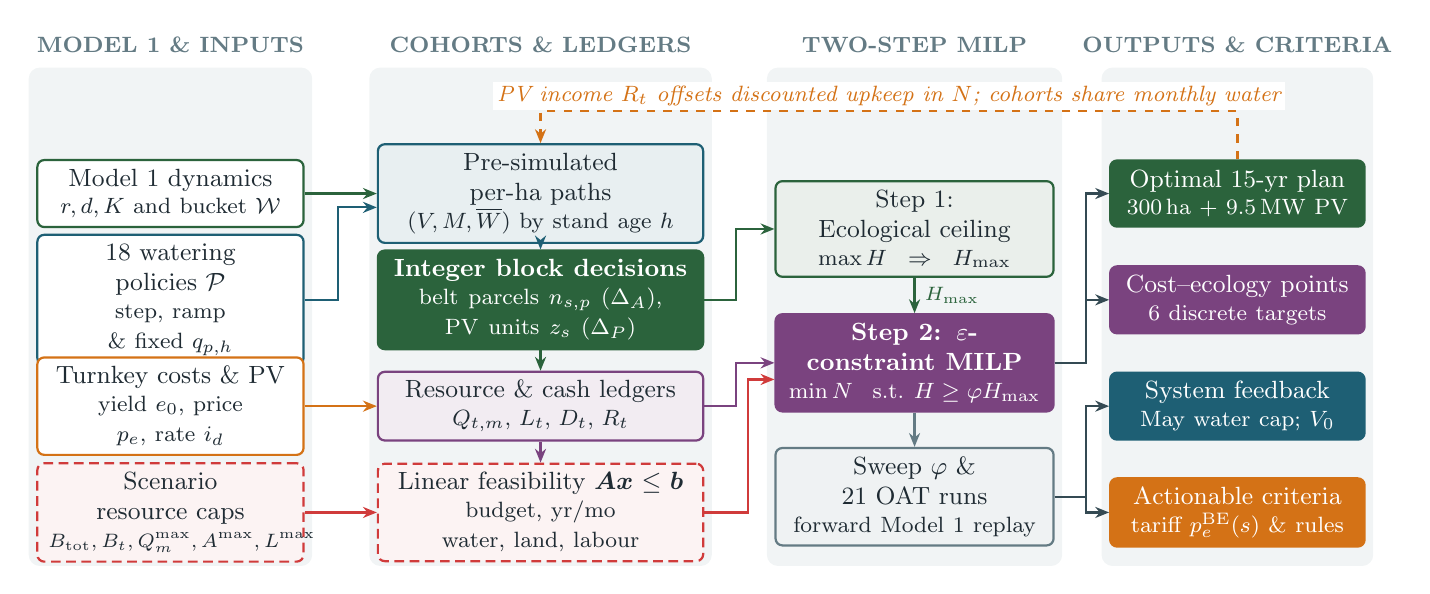
\begin{tikzpicture}
% ---- column headings
\node[colhead] at (1.90,0.72)  {MODEL 1 \& INPUTS};
\node[colhead] at (6.60,0.72)  {COHORTS \& LEDGERS};
\node[colhead] at (11.35,0.72) {TWO-STEP MILP};
\node[colhead] at (15.45,0.72) {OUTPUTS \& CRITERIA};

% ---- column 1: inputs (y = -0.95, -2.30, -3.65, -5.00)
\node[data=pVeg,   text width=3.1cm] (m1)   at (1.90,-0.95) {Model 1 dynamics\\[-1pt]{\footnotesize $r,d,K$ and bucket $\mathcal W$}};
\node[data=pWater, text width=3.1cm] (pol)  at (1.90,-2.30) {18 watering policies $\mathcal P$\\[-1pt]{\footnotesize step, ramp \& fixed $q_{p,h}$}};
\node[data=pPV,    text width=3.1cm] (cost) at (1.90,-3.65) {Turnkey costs \& PV\\[-1pt]{\footnotesize yield $e_0$, price $p_e$, rate $i_d$}};
\node[capbox,      text width=3.1cm] (caps) at (1.90,-5.00) {Scenario resource caps\\[-1pt]{\scriptsize $B_{\mathrm{tot}},B_t,Q_m^{\max},A^{\max},L^{\max}$}};

% ---- column 2: cohorts & ledgers
\node[step=pWater, text width=3.85cm] (pre) at (6.60,-0.95) {Pre-simulated per-ha paths\\[-1pt]{\footnotesize $(V,M,\overline W)$ by stand age $h$}};
\node[core=pVeg,   text width=3.85cm] (dec) at (6.60,-2.30) {Integer block decisions\\[-1pt]{\footnotesize\normalfont belt parcels $n_{s,p}$ ($\Delta_A$), PV units $z_s$ ($\Delta_P$)}};
\node[step=pPlum,  text width=3.85cm] (led) at (6.60,-3.65) {Resource \& cash ledgers\\[-1pt]{\footnotesize $Q_{t,m},\,L_t,\,D_t,\,R_t$}};
\node[capbox,      text width=3.85cm] (chk) at (6.60,-5.00) {Linear feasibility $\bm A\bm x\le\bm b$\\[-1pt]{\footnotesize budget, yr/mo water, land, labour}};

% ---- column 3: two-step MILP
\node[step=pVeg,      text width=3.25cm] (s1)  at (11.35,-1.40) {Step 1: Ecological ceiling\\[-1pt]{\footnotesize $\max H \;\Rightarrow\; H_{\max}$}};
\node[core=pPlum,     text width=3.25cm, minimum height=1.08cm] (s2) at (11.35,-3.10) {Step 2: $\varepsilon$-constraint MILP\\[-1pt]{\footnotesize\normalfont $\min N$ \ s.t.\ $H\ge\varphi H_{\max}$}};
\node[step=pGreyDark, text width=3.25cm] (oat) at (11.35,-4.80) {Sweep $\varphi$ \& 21 OAT runs\\[-1pt]{\footnotesize forward Model 1 replay}};

% ---- column 4: outputs
\node[result=pVeg,   text width=2.95cm] (plan)  at (15.45,-0.95) {Optimal 15-yr plan\\[-1pt]{\footnotesize 300\,ha + 9.5\,MW PV}};
\node[result=pPlum,  text width=2.95cm] (front) at (15.45,-2.30) {Cost--ecology points\\[-1pt]{\footnotesize 6 discrete targets}};
\node[result=pWater, text width=2.95cm] (fb)    at (15.45,-3.65) {System feedback\\[-1pt]{\footnotesize May water cap; $V_0$}};
\node[result=pPV,    text width=2.95cm] (rule)  at (15.45,-5.00) {Actionable criteria\\[-1pt]{\footnotesize tariff $p_e^{\mathrm{BE}}(s)$ \& rules}};

% ---- flows
\draw[flow=pVeg]   (m1.east)   -- (pre.west);
\draw[flow=pWater] (pol.east)  -- ++(0.42,0) |- ([yshift=-5pt]pre.west);
\draw[flow=pWater] (pre.south) -- (dec.north);
\draw[flow=pPV]    (cost.east) -- (led.west);
\draw[flow=pVeg]   (dec.south) -- (led.north);
\draw[flow=pPlum]  (led.south) -- (chk.north);
\draw[flow=pLimit] (caps.east) -- (chk.west);

\draw[flow=pVeg]   (dec.east)  -- ++(0.40,0) |- (s1.west);
\draw[flow=pPlum]  (led.east)  -- ++(0.40,0) |- (s2.west);
\draw[flow=pLimit] (chk.east)  -- ++(0.56,0) |- ([yshift=-6pt]s2.west);
\draw[flow=pVeg]   (s1.south)  -- node[right, font=\scriptsize\bfseries, text=pVeg] {$H_{\max}$} (s2.north);
\draw[flow=pGreyDark] (s2.south) -- (oat.north);

\draw[flow] (s2.east)  -- ++(0.40,0) |- (plan.west);
\draw[flow] (s2.east)  -- ++(0.40,0) |- (front.west);
\draw[flow] (oat.east) -- ++(0.40,0) |- (fb.west);
\draw[flow] (oat.east) -- ++(0.40,0) |- (rule.west);

% ---- clean orthogonal top coupling arc (clear above every box)
\draw[flow=pPV, dashed] (plan.north) -- (15.45, 0.10)
  -- node[above, font=\footnotesize\itshape, text=pPV, fill=white, inner sep=1.5pt]
     {PV income $R_t$ offsets discounted upkeep in $N$; cohorts share monthly water}
  (6.60, 0.10) -- (pre.north);

% ---- light column bands
\begin{scope}[on background layer]
  \foreach \x/\w in {1.90/3.6, 6.60/4.35, 11.35/3.75, 15.45/3.45}
    \fill[pGrid!55, rounded corners=4pt] (\x-\w/2,0.65) rectangle (\x+\w/2,-5.68);
\end{scope}
\end{tikzpicture}
\end{document}
